\section{Непрерывность вероятностной меры}

\begin{definition}
    $(\Omega,\mathcal{F},\Pr)$ --- вероятностная (колмогоровская)
    тройка, или вероятностное пространство.
\end{definition}

\begin{definition}[1. $\sigma$-аддитивность]
    Мера $\Pr$ называется \textbf{$\sigma$-аддитивной}, если
    для попарно непересекающихся $A_i\in\mathcal{F}$
    \[
        \Pr\left(\bigsqcup_{i=1}^{\infty}A_i\right)
        =\sum_{i=1}^{\infty}\Pr(A_i).
    \]
\end{definition}

\begin{definition}[2. Непрерывность снизу]
    Мера $\Pr$ называется \textbf{непрерывной снизу}, если
    для любой неубывающей последовательности
    $A_i\in\mathcal{F}$, $A_i\subset A_{i+1}$,
    \[
        A=\bigcup_{i=1}^{\infty}A_i
        \quad\Longrightarrow\quad
        \Pr(A)=\lim_{i\to\infty}\Pr(A_i).
    \]
\end{definition}

\begin{center}
    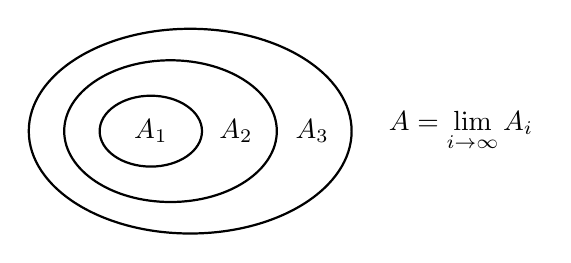
\begin{tikzpicture}
        \draw[thick] (0,0) ellipse (0.65cm and 0.45cm);
        \draw[thick] (0.25,0) ellipse (1.35cm and 0.9cm);
        \draw[thick] (0.5,0) ellipse (2.05cm and 1.3cm);
        \node at (0,0) {$A_1$};
        \node at (1.08,0) {$A_2$};
        \node at (2.05,0) {$A_3$};
        \node[right] at (2.9,0)
            {$A=\lim\limits_{i\to\infty}A_i$};
    \end{tikzpicture}
\end{center}

\begin{definition}[3. Непрерывность сверху]
    Мера $\Pr$ называется \textbf{непрерывной сверху}, если
    для любой невозрастающей последовательности
    $B_i\in\mathcal{F}$, $B_i\supset B_{i+1}$,
    \[
        B=\bigcap_{i=1}^{\infty}B_i
        \quad\Longrightarrow\quad
        \Pr(B)=\lim_{i\to\infty}\Pr(B_i).
    \]
\end{definition}

\begin{theorem}
    Для вероятностной меры на $\sigma$-алгебре условия
    1, 2 и 3 эквивалентны:
    \[
        \text{$\sigma$-аддитивность}
        \quad\Longleftrightarrow\quad
        \text{непрерывность снизу}
        \quad\Longleftrightarrow\quad
        \text{непрерывность сверху}.
    \]
\end{theorem}

\begin{Proof}[$1\implies3$]
    Пусть $B_i\supset B_{i+1}$. Положим
    \[
        A_i=B_i\setminus B_{i+1},
        \qquad B=\bigcap_{i=1}^{\infty}B_i.
    \]
    \begin{center}
        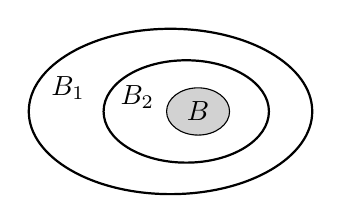
\begin{tikzpicture}
            \draw[thick] (0,0) ellipse (1.8cm and 1.05cm);
            \draw[thick] (0.2,0) ellipse (1.05cm and 0.65cm);
            \fill[gray!35] (0.35,0) ellipse (0.4cm and 0.3cm);
            \draw (0.35,0) ellipse (0.4cm and 0.3cm);
            \node at (-1.3,0.3) {$B_1$};
            \node at (-0.42,0.18) {$B_2$};
            \node at (0.35,0) {$B$};
        \end{tikzpicture}
    \end{center}
    Имеем
    \[
        \left(\bigsqcup_{i=1}^{\infty}A_i\right)\sqcup B=B_1.
    \]
    По $\sigma$-аддитивности
    \[
        \sum_{i=1}^{\infty}\Pr(A_i)+\Pr(B)=\Pr(B_1),
        \qquad \Pr(A_i)=\Pr(B_i)-\Pr(B_{i+1}).
    \]
    Следовательно,
    \[
        \lim_{n\to\infty}
        \underbrace{\sum_{i=1}^{n}
        \bigl(\Pr(B_i)-\Pr(B_{i+1})\bigr)}
        _{\Pr(B_1)-\Pr(B_{n+1})}
        +\Pr(B)=\Pr(B_1).
    \]
    Значит,
    \[
        \Pr(B_1)-\lim_{n\to\infty}\Pr(B_{n+1})
        +\Pr(B)=\Pr(B_1),
    \]
    откуда $\Pr(B)=\lim_{n\to\infty}\Pr(B_{n+1})$.
\end{Proof}
